% !TEX root = comparison.tex
\section{Experimental Setup}
We want two discuss two applications, in which we are making use of lineups to compare competing designs. 
The first one arises from a discussion of how wind direction affects efficiency of an airport. In this example, we are dealing with all flights \cite{rita} in and out of Seattle/Tacoma International Airport (SEA) between July 2008 and June 2011. As a measure of airport efficiency we are using time between successive wheel-events (time at wheel take-off or touch-down), which we found to be independent of airline carrier and operating hours, as long as we restricted the data to `regular' operating hours between 7 am and midnight and `regular' weather conditions -- i.e. we eliminated records associated with the top 5\% wind speed measurements \cite{noaa-weather}, leaving us with just under 0.5 Million flights.

Statistical tests of mean efficiency by wind direction are not particularly helpful in this situation:
the difference in mean efficiency between the most efficient wind direction and the least efficient shows a statistically significant difference with a $p$-value $\le 10^{15}$. %2.2e-16$. 
However, out of the 34 other wind directions,  another 31 show significant differences in efficiency as well. This is much more a property of the large data size rather than practically usable differences. Mere significances also do not allow us an assessment of the underlying pattern.

\subsection{Wind Direction and Airport Efficiency}
In deciding on the design for displaying efficiency  by wind direction we were using the fact that wind direction is circular, and  displayed the data as (conditional) wind rose charts - i.e. for each of 36 wind directions we show the percentage of flights falling into one-minute intervals between successive flights, from  0 minutes to 8 minutes or more.


\begin{figure}[htbp] %  figure placement: here, top, bottom, or page
%   \centering
 \hspace{-.1in}
   \begin{tabular}{ccl}
   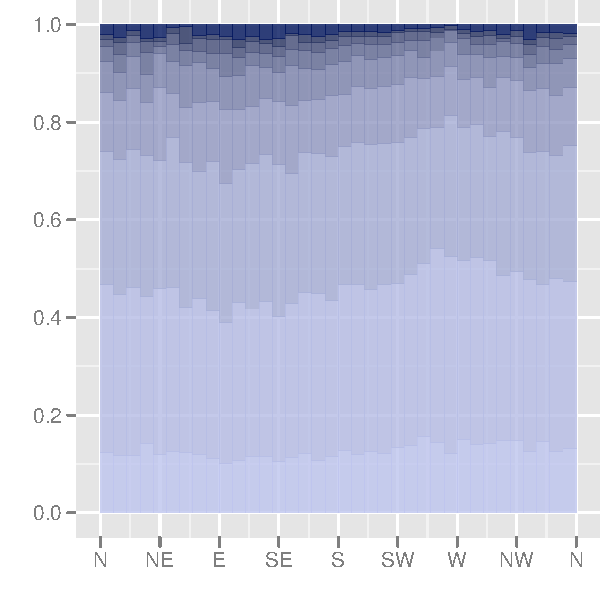
\includegraphics[width=0.375\linewidth]{euclid_noline.pdf} & \hspace{-.3in}
   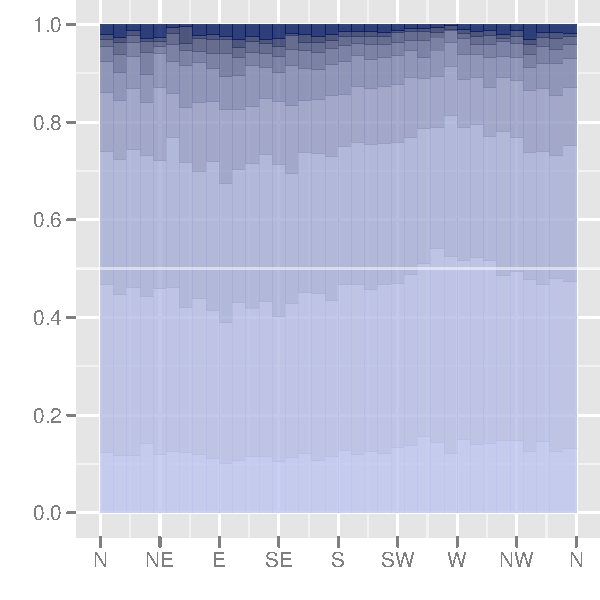
\includegraphics[width=0.375\linewidth]{euclid_line.pdf} &  \hspace{-.2in} \multirow{2}{*}[.55in]{  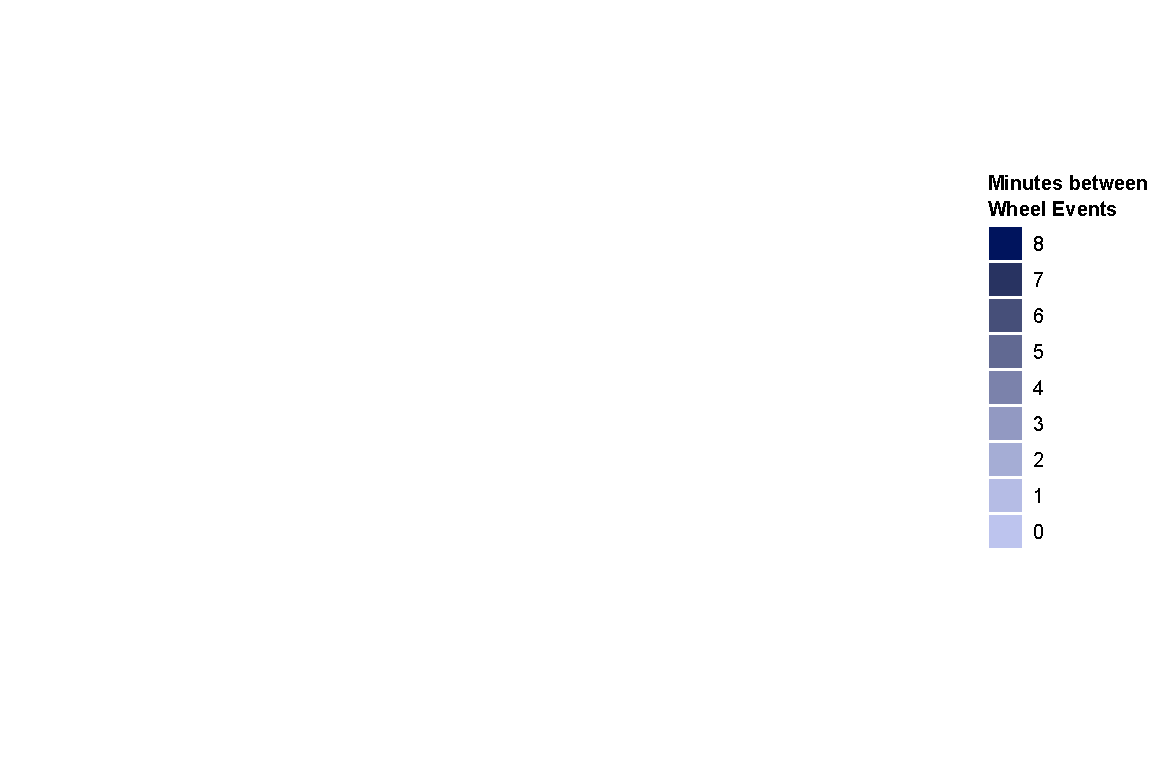
\includegraphics[width=0.2\linewidth]{legend.pdf}} \\
   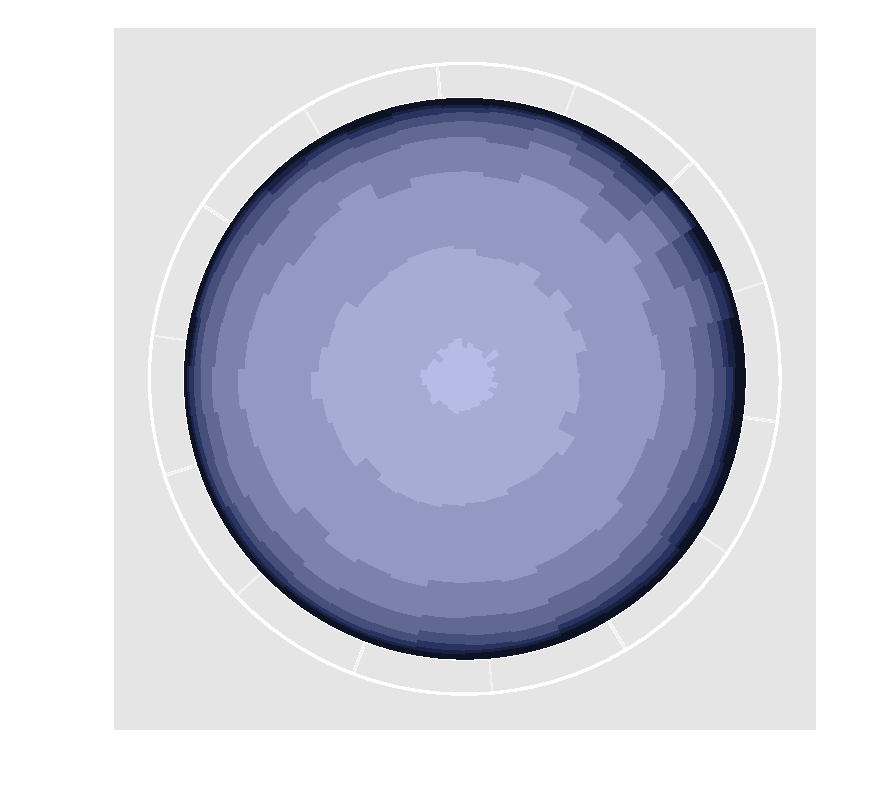
\includegraphics[width=0.43\linewidth]{Polar_NoLine.pdf} &  \hspace{-.3in}
   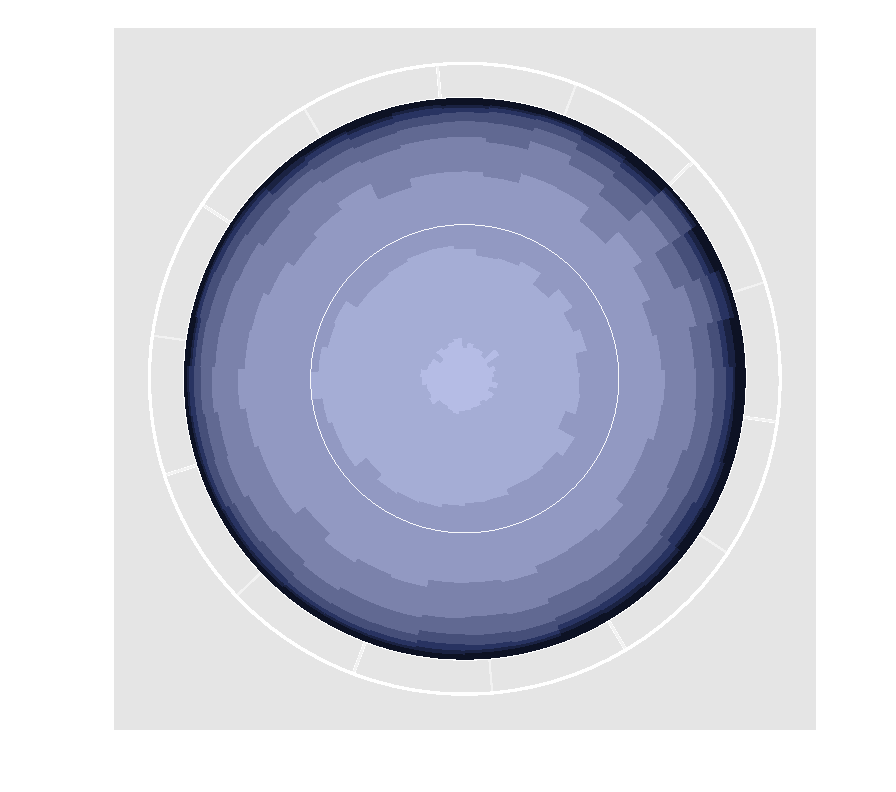
\includegraphics[width=0.43\linewidth]{Polar_Line.pdf}  
   \end{tabular}
   \caption{All four competing designs: polar versus Euclidean charts in top and bottom row, with (right) and without (left) reference lines at 50\%. }
   \label{layouts}
\end{figure}

In spite of the contextual circular property of wind direction, the pattern in efficiency did not seem to stand out well during the exploration process, which led us to using a corresponding  Euclidean design. Both designs were additionally equipped with a reference line at 50\%. 
Figure \ref{layouts} shows an overview of all four chart types in the study. During the exploration of the data, it became clear that Seattle airport functions at it best with winds coming from the East to Southeast, while winds from the West seemed to be most troublesome. Since runways can be used in both directions, changing the runway usage according to dominant wind direction for that day or time of the year might be a feasible solution in gaining efficiency. 

\begin{figure}[htbp] %  figure placement: here, top, bottom, or page
   \centering

\begin{tabular}{cl}
\phantom{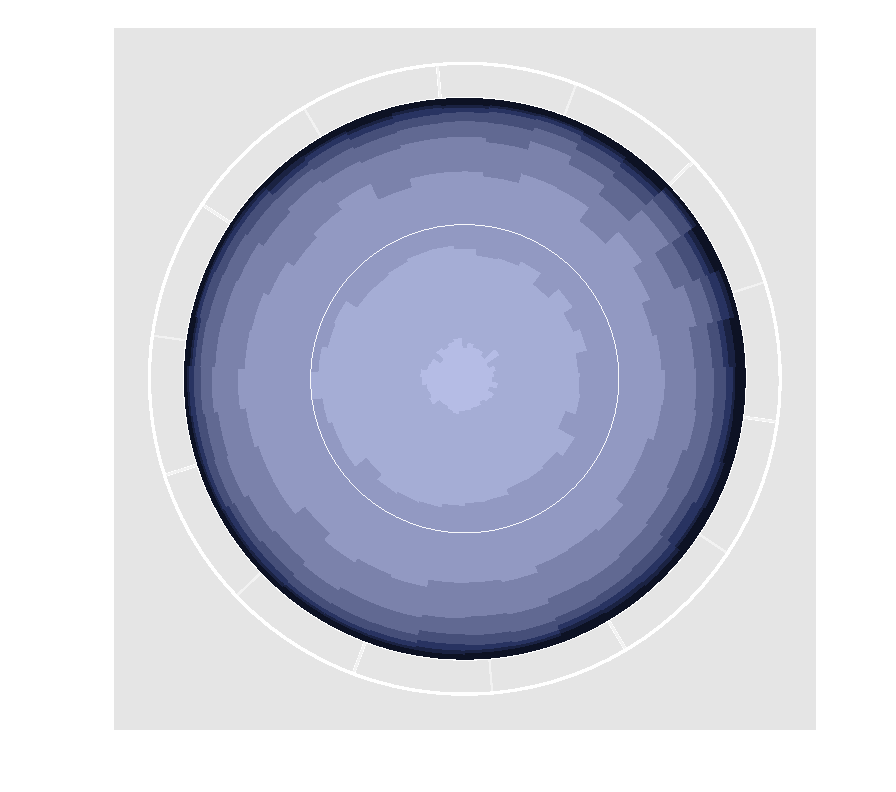
\includegraphics[width=0.03\linewidth]{Polar_Line.pdf}} & \vspace{-0.035in} \multirow{10}{*}{\hspace{-0.25in}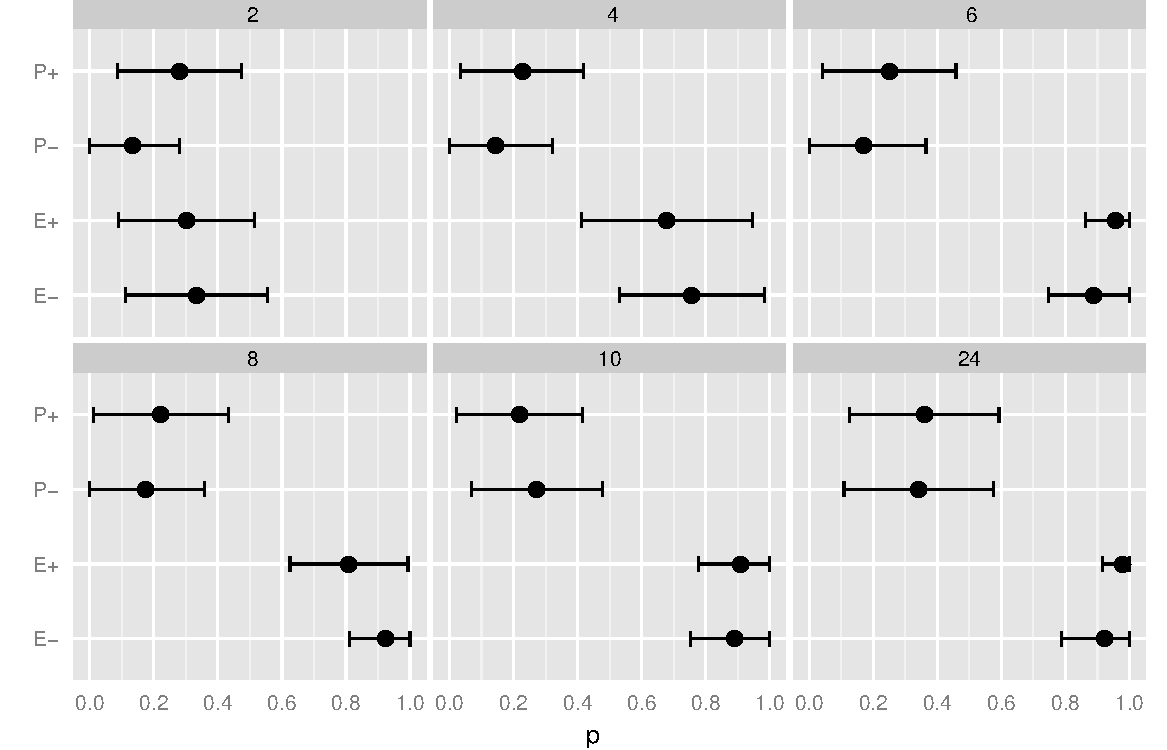
\includegraphics[width=0.9\linewidth]{turk4-designs.pdf}} \\
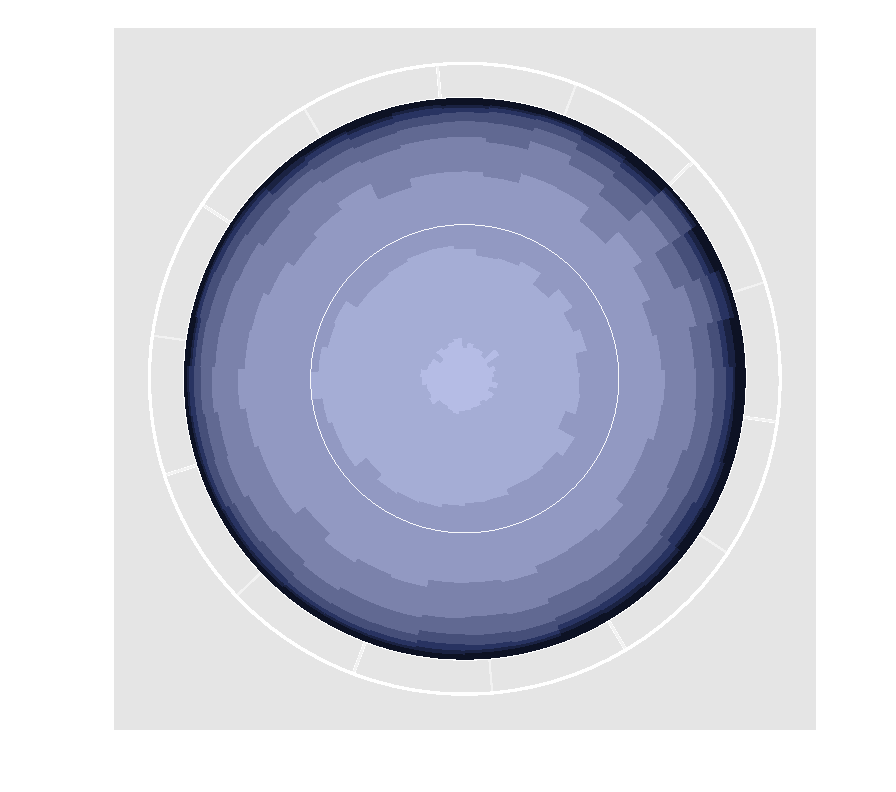
\includegraphics[width=0.055\linewidth]{Polar_Line.pdf} \\
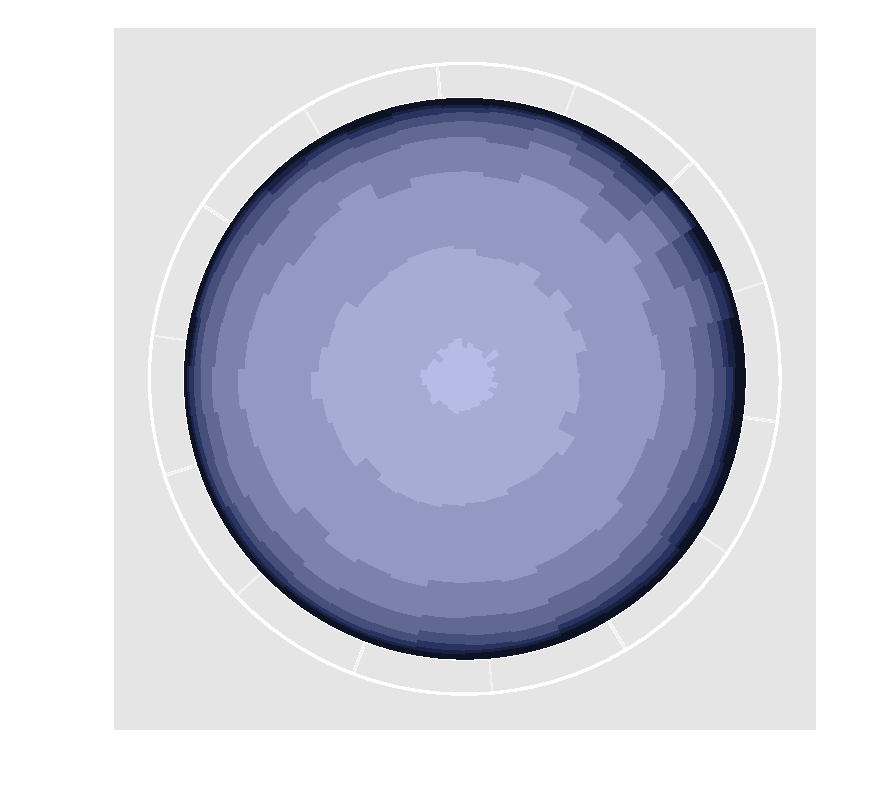
\includegraphics[width=0.055\linewidth]{Polar_NoLine.pdf} \\
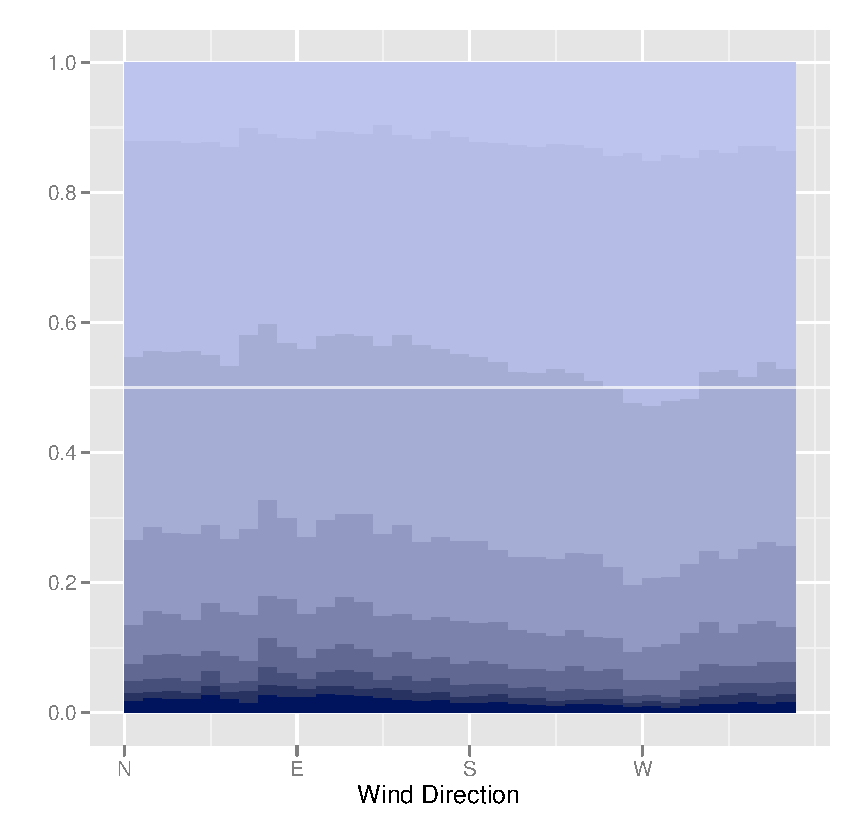
\includegraphics[width=0.045\linewidth]{Euclidian_Line.pdf} \\
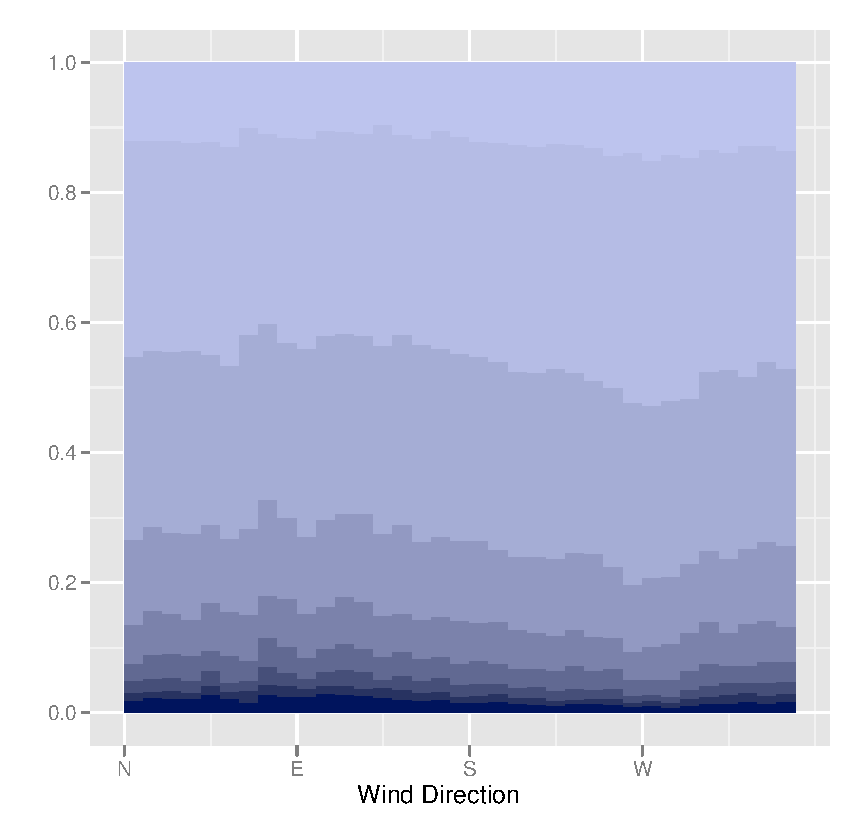
\includegraphics[width=0.045\linewidth]{Euclidian_NoLine.pdf}\\
\phantom{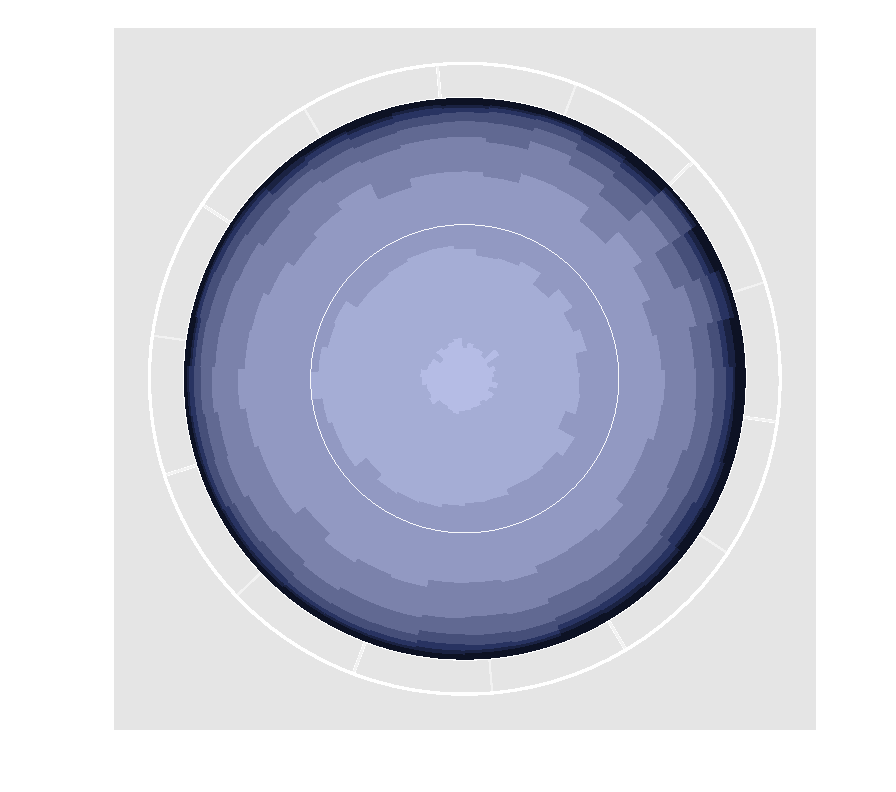
\includegraphics[width=0.03\linewidth]{Polar_Line.pdf}}\\
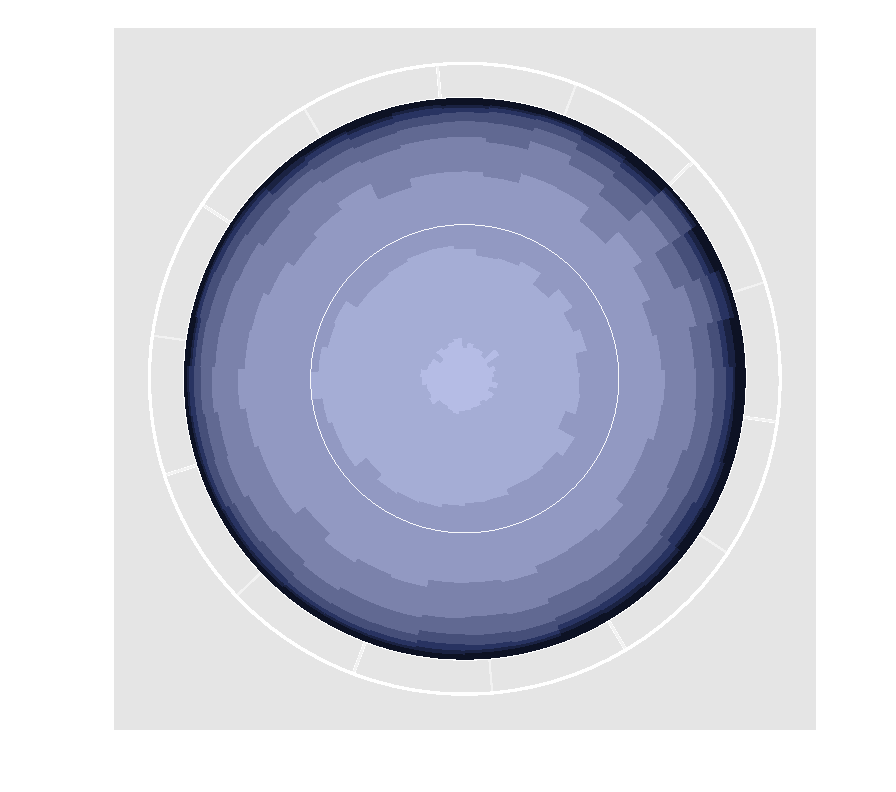
\includegraphics[width=0.055\linewidth]{Polar_Line.pdf} \\
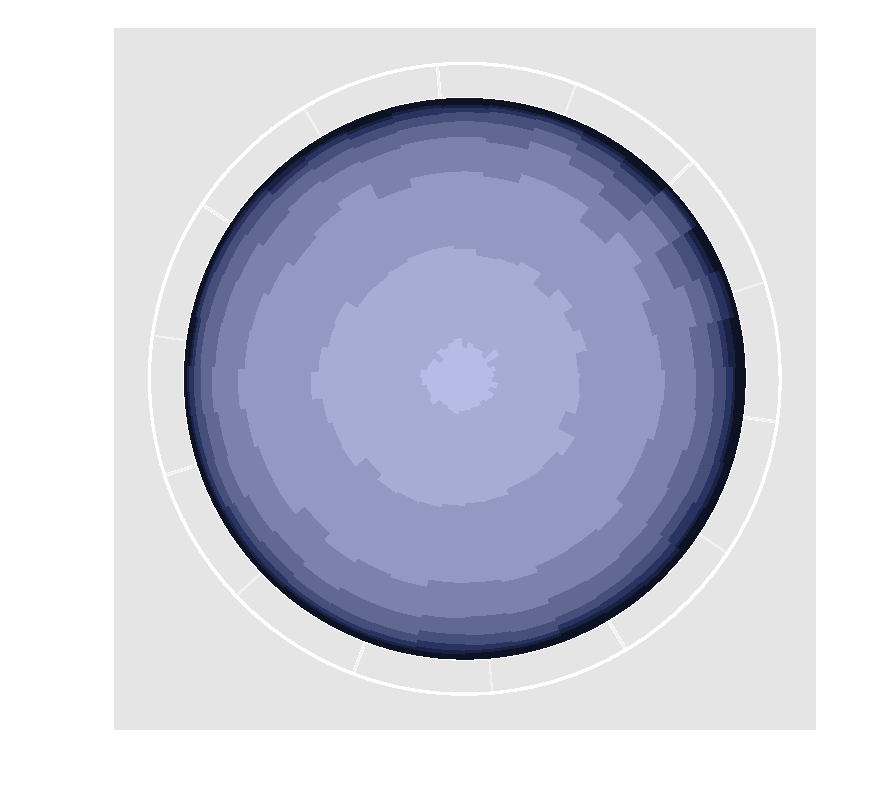
\includegraphics[width=0.055\linewidth]{Polar_NoLine.pdf} \\
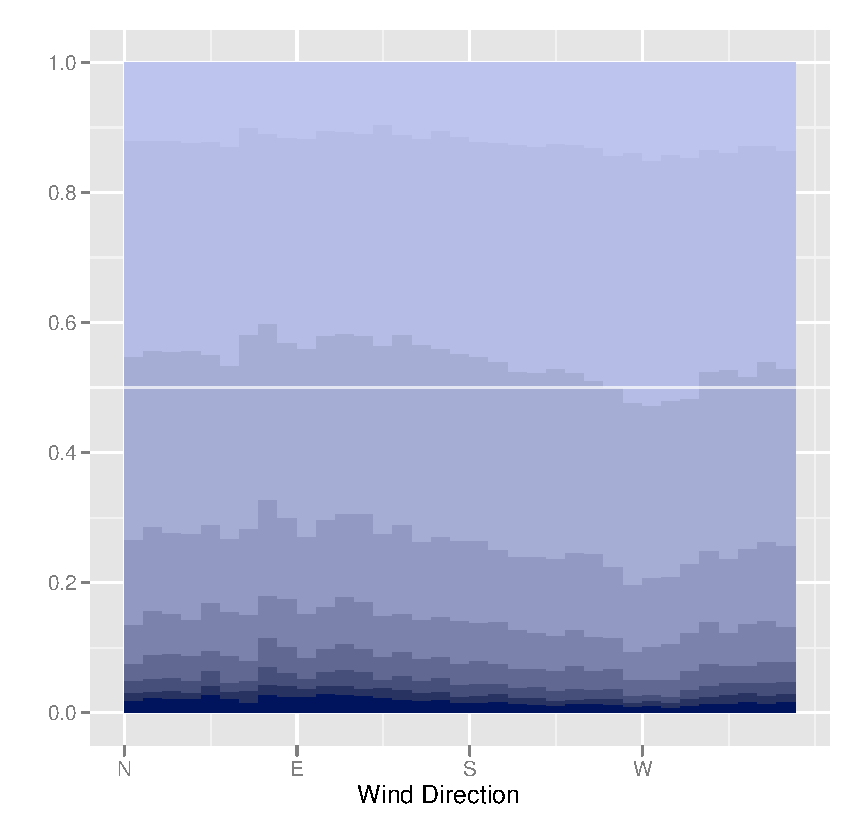
\includegraphics[width=0.045\linewidth]{Euclidian_Line.pdf} \\
      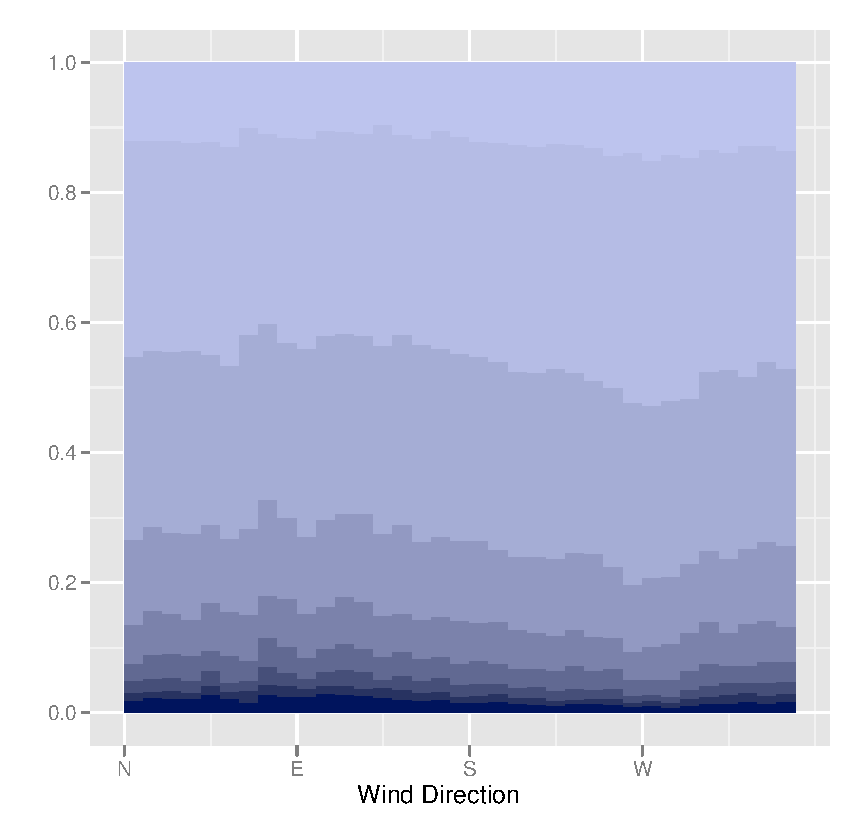
\includegraphics[width=0.045\linewidth]{Euclidian_NoLine.pdf}
  \end{tabular} 
  \vspace{0.1in}
   \caption{Power results for two competing designs: polar versus a Euclidean, with and without a reference line. Error bars indicate 95\% confidence intervals. Plots are facetted by percentage of data used. }
   \label{fig:example}
\end{figure}

An additional factor we were interested in this particular situation was to assess, how much of the data we actually needed to use in a design to have observers pick out the pattern. Clearly, a design is more efficient, if a smaller sample size is sufficient for showing the presence of a relationship. In order to investigate this, we took different size samples of the data and created lineup plots of all four designs for these subsets. Another perturbation is to 
That also allows us to get multiple responses from each observer to assess individual ability. 


Describe the experimental setup: polar charts versus euclidean - with and without reference lines.
Figure showing all four types using the same dataset. 
Discuss construction of each one. Discuss construction of null chart.

The goal of this experiment is to understand the efficiency of displaying information using euclidian and polar coordinates. Efficiency is the deviation from independence, which can be simulated by taking permutations of the original dataset. Data concerning wind patterns and time between flights at SEA airport is used for these charts. The lineup chart is composed of 20 graphics with all of the exact same characteristics except for the data. One of the 20 graphics will be using original airport data while the other 19 will be permutations of that data. Efficiency of the chart types can be inferred by how accurately individuals pick out the plot with the original data. There are other variables which are introduced to further our understanding of the way we perceive euclidian and polar coordinates. All combinations of each level of the variables are involved in the experiment for both polar and euclidian coordinates. The graphics in each chart will all have exactly the same level of the variables with the only difference being the data. 

The other variables which are monitored are existence of reference line, placement of x-axis, and sample size. It is possible that one of the chart types benefits more from additional components such as reference lines. The polar and euclidian null charts will be shown either with or without a white reference line. The line is placed at slightly over 50 percent of the y axis. Additionally, the x-axis has four placements. The original dataset contains a characteristic wave pattern, which for euclidian coordinates, may be a large factor contributing to the perceived effectiveness of the graphic. Characteristic patterns such as the wave pattern may be perceived in a different way when viewed in polar coordinates. When the x-axis is is shifted the look of the pattern changes. The wave pattern is broken up for euclidian coordinates but for polar coordinates is only shifted around the axis. Finally, the amount of information necessary for detection as well as correctness is a measure for efficiency of the charts so the sample size which was taken from the original dataset is of interest. The original data set contained XXX,XXX observations from which 2, 4, 6, 8, 10, and 24 percent of the observations were sampled. Small sample sizes are easier to obtain because of time and money constraints. It would be nice to know if there is one type of chart which can show data trends using less information. 


 All combinations of these variables were repeated for plots with a reference line and without a reference line, as shown in figure \ref{layouts}.This figure shows examples of graphics showing the actual data, which in the experiment would be randomly positioned among 19 null plots. In total there are XXX unique charts which represent all different combinations of sample size, coordinate type, x-axis placement, and whether or not there is a reference line. The charts are all assigned a difficulty level, which is based on sample size, on a scale from zero to four. There are two plots assigned a difficulty level of zero. These two charts, one polar and one Euclidian, were made from computer generated data and intended to be at the level where an individual, if he or she is not purely guessing, should be able to find the correct plot. 


Amazon's Mechanical Turk is an online service in which individuals can request and perform simple tasks and surveys for money. Using Turk we were able to gather data on how people responded to the charts. Each person is shown a series of ten charts and asked to choose the graphic on each chart which they think is "different". They then identify, from a list of choices, why they chose this particular chart as well as how confident they are on a scale of one to five. Personal information such as age group, gender, and education is also collected on a voluntary basis. The amount of time it took the individual to answer is also recorded. This study allows us to make informed judgments about how the plot type effects efficiency in terms of accuracy and time spent reading the plots. Xcite stephen few?X

Effect is deviation from independence. Cannot be properly measured statistically except in highly aggregated situations, where the effect might be washed out.

Most generally this experiment can be paralleled to the pie chart versus barchart discussion. The Euclidian coordinate plot is made up of bars *whose?* areas are colored proportionally according to the data. The polar coordinate plot is made up of pie slices which are also colored proportionally according to the data. Viewers of these charts will visually decode the areas of the bars and pie slices and make a judgement based on their decoding. How accurate this judgment is is left to be discussed. According to  \citet[page=40]{kosslyn:2006}, area is usually perceived as a function of what the actual area is. This function is the area raised to an exponent of approximately 0.8 and then multiplied by a constant. However, when bars are parallel, the relative height of these bars is perceived very accurately. From this information, one could infer that the Euclidian coordinate plot may gain efficiency based on the height of the colored bars. 


Pie versus Barchart discussion is pretty old: cite some of the literature:

From Stephen Few, perceptual edge:
	When a graph is made, quantitative and categorical information is encoded by a display method. Then the information is visually decoded. This visual perception is a vital link. No matter how clever the choice of the information, and no matter how technologically impressive the encoding, a visualization fails if the decoding fails. Some display methods lead to efficient, accurate decoding, and others lead to inefficient, inaccurate decoding. It is only through scientific study of visual perception that informed judgments can be made about display methods. (William S. Cleveland, The Elements of Graphing Data, Hobart Press, 1994, p. 1)
	
	The systematic distortion of area is captured by �Steven�s Power Law,� which states that the psychological impression is a function of the actual physical magnitude raised to an exponent (and multiplied by a scaling constant). To be precise, the perceived area is usually equal to the actual area raised to an exponent of about 0.8, times a scaling constant...In contrast, relative line length [such as the lengths of bars] is perceived almost perfectly, provided that the lines are oriented the same way \cite[page=40]{kosslyn:2006}
	
	
	We make angle judgments when we read a pie chart, but we don�t judge angles very well. These judgments are biased; we underestimate acute angles (angles less than 90�) and overestimate obtuse angles (angles greater than 90�). Also, angles with horizontal bisectors (when the line dividing the angle in two is horizontal) appear larger than angles with vertical bisectors. (Naomi Robbins, Creating More Effective Graphs, Wiley, 2005, p. 49)
	
	 Edward Tufte once said that �the only worse design than a pie chart is several of them, for then the viewer is asked to compare quantities located in spatial disarray both within and between pies� (Edward Tufte, The Visual Display of Quantitative Information, Graphics Press, 1983, p. 178.)

 We do not claim to settle the question - which is multi-facetted and will not have a clear 'winning' design but instead very much depends on the purpose of the chart and task at hand.

